
\begin{tcolorbox}[colback=white!10!white,colframe=green!30!black,title=Kompensator] 
Das ist die Kombination aus einem Regler und Beobachter. Die beiden werden separat entworfen und anschließend zu einem System zusammengefasst.
\begin{figure}[H]
\centering
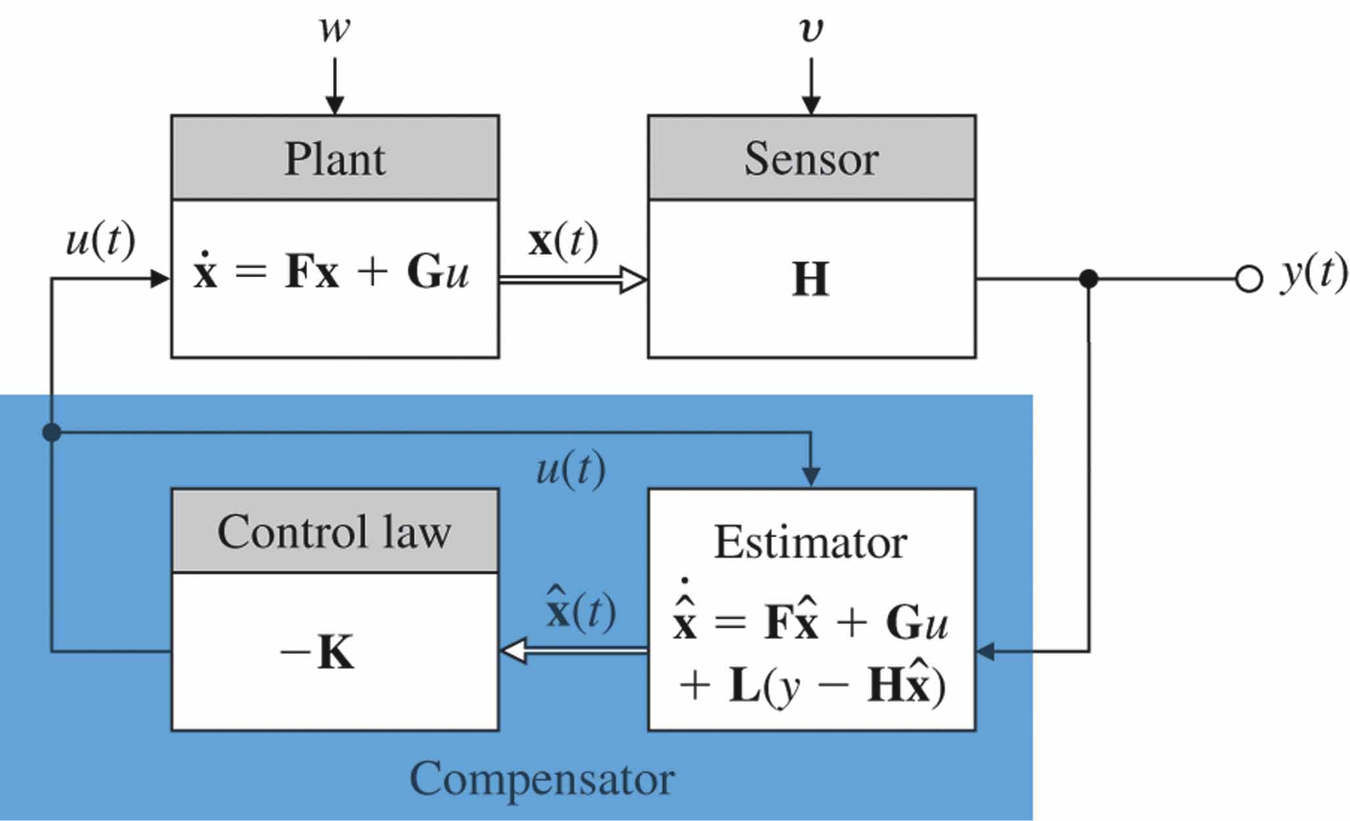
\includegraphics[width=0.7\linewidth]{content/img/kompensator}
\caption{}
\label{fig:kompensator}
\end{figure}
Übertragungsfunktion lässt sich berechnen durch:
\begin{align*}
    &D(s) = \frac{U(s)}{Y(s)}\\
    &U(s) = \det(P(s)) = \det\left[\begin{array}{l|r}
    s\bs{I}- \bs{A} & \bs{L}\\\hline
    \bs{K} & 0
    \end{array}\right]\\
    &Y(s) = \det(s\bs{I}-\bs{F}+\bs{LH}+\bs{GK})
\end{align*} 

\end{tcolorbox}
